%!TEX root = ./main.tex

\chapter{Ports details}

\section{PowerPC}

\subsection{System services} \label{sec:systemservices}

The PowerPC port uses the \asfct{sc} software interrupt to call system services \cite{mpc32bsc}. \asfct{sc} stands for System Call. It saves the current \reg{PC} in \reg{SRR0} register and the current \reg{MSR} in \reg{SRR1} register and jump to the System Call handler.

The id of the system service to call is given in the \reg{r0} register and \reg{r0} save and restore are added around. For instance, the following listing gives the \api{ActivateTask} service code. These function are generated from templates by goil (see \ref{sec:generatedfiles}) and are part of the {\em invoque} layer (see \ref{sec:invoque}):

\begin{lstlisting}[language=C]
  .global ActivateTask
ActivateTask:
  subi r1,r1,4                       /* make room on stack    */
  stw  r0,0(r1)                      /* save r0               */
  li   r0,OSServiceId_ActivateTask   /* load r0 with the id   */
  sc                                 /* system call           */
  lwz  r0,0(r1)                      /* restore r0            */
  addi r1,r1,4                       /* restore stack         */
  blr                                /* return                */
  
  .type ActivateTask,@function
  .size ActivateTask,$$-ActivateTask
\end{lstlisting}

When the System Call begin execution, the process stack has the mapping depicted in figure \ref{fig:stackbeginningSC}.

\begin{figure}[htbp] %  figure placement: here, top, bottom, or page
\begin{minipage}{0.5\textwidth}
    \centering
  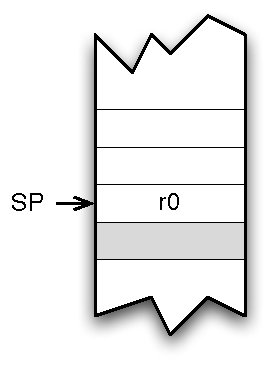
\includegraphics[scale=.6]{pictures/PStackAfterInvoque} 
\end{minipage}
\begin{minipage}{0.5\textwidth}
   \caption{Process stack mapping at the beginning of the System Call handler. The grayed zone represents an unknown content depending on from where the service was called.}\label{fig:stackbeginningSC}
\end{minipage}
\end{figure}

\subsection{Dispatching the service call}

The System Call handler is usually located in the \hex{0C00} exception handler but, depending on the CPU kind, it may be located elsewhere. Since the available memory for the interrupt or exception handler may vary, a jump is made to the \cfunction{tpl_sc_handler}.%:

%\begin{lstlisting}
%  .section  .SC_vector  CODE_ACCESS_RIGHT
%tpl_sc_vector:
%  b   tpl_sc_handler
%
%  .section  .SC_handler CODE_ACCESS_RIGHT
%\end{lstlisting}

\cfunction{tpl_sc_handler} performs the following tasks:
\begin{penum}
\item saves additional registers to be able to work
\item disables memory protection
\item switches to kernel stack if needed
\item calls the service
\item performs a context switch if needed and programs the MPU.
\item switches back to the process stack if needed
\item enable memory protection
\item restore registers
\item get back to the process
\end{penum}

\note{Currently the PowerPC port does not support tasks that use floating point registers}

\subsubsection{Saving additional registers}

The following registers are saved: \var{lr}, \var{cr}, \var{r11} and \var{r12}. In fact, it should be not necessary to save \var{r11} and \var{r12} because these registers are volatile as defined in the PowerPC EABI \cite{PPCeabi} but we prefer a conservative approach. Register saving is done by the following code at start of the \cfunction{tpl_sc_handler} and the mapping of the process stack is depicted at figure \ref{fig:stackSavingSC}:

\begin{lstlisting}[language=C]
  subi  r1,r1,PS_FOOTPRINT  /* Make room on stack */

  stw   r11,PS_R11(r1)      /* Save r11           */
  stw   r12,PS_R12(r1)      /* Save r12           */
  mflr  r11
  stw   r11,PS_LR(r1)       /* Save lr            */
  mfcr  r11
  stw   r11,PS_CR(r1)       /* Save cr            */
\end{lstlisting}

\begin{figure}[htbp] %  figure placement: here, top, bottom, or page
\begin{minipage}{0.5\textwidth}
    \centering
  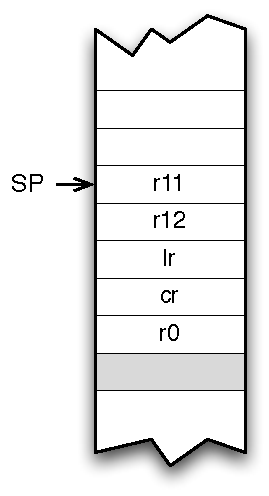
\includegraphics[scale=.6]{pictures/PStackAfterSCSaving} 
\end{minipage}
\begin{minipage}{0.5\textwidth}
   \caption{Process stack mapping after additional registers have been saved by the beginning of the System Call handler.}\label{fig:stackSavingSC}
\end{minipage}
\end{figure}

\subsubsection{Disabling memory protection}

This part of the dispatch layer is done in the \cfunction{tpl_enter_kernel} function and is assembled only if \cmacro{WITH_MEMORY_PROTECTION} is set to \YES. After saving the \reg{lr}, the \cfunction{tpl_kernel_mp} function is called and does the actual job. At last \reg{lr} is restored.

\begin{lstlisting}[language=C]
#if WITH_MEMORY_PROTECTION == YES
  /*
   * Switch to kernel mem protection scheme
   */
  subi  r1,r1,4
  mflr  r11
  stw   r11,0(r1)       /* save lr on the current stack */
  bl    tpl_kernel_mp   /* disable memory protection    */
  lwz   r11,0(r1)       /* restore lr                   */
  mtlr  r11
  addi  r1,r1,4
#endif
\end{lstlisting}

\subsubsection{Switching to the kernel stack}

Once the dispatch layer has saved the registers it uses and has switched to the kernel memory protection scheme, it switches to the kernel stack. However the kernel stack could used already because a call to a \cfunction{PreTaskHook} or a \cfunction{PostTaskHook} is done on the kernel stack and such a hook may call a service. So the dispatch layer is reentrant. The number of reentrant calls is counted by the \var{tpl_reentrancy_counter}. In addition the process stack pointer (\reg{r1}), \reg{SRR0} and \reg{SRR1} are saved in the kernel stack. The kernel stack mapping is shown in figure \ref{fig:kernelstackmapping}. For a reentrant call, the same frame is build over the current one. The switch to the kernel stack is done as follow:

\begin{lstlisting}[language=C]
  /*
   * Check the reentrency counter value and increment it
   * if the value is 0 before the inc, then we switch to
   * the system stack.
   */
  lis   r11,TPL_HIG(tpl_reentrancy_counter)
  ori   r11,r11,TPL_LOW(tpl_reentrancy_counter)
  lwz   r12,0(r11)    /* get the value of the counter */
  cmpwi r12,0
  addi  r12,r12,1
  stw   r12,0(r11)
  bne   no_stack_change
  
  /*
   * Switch to the kernel stack
   *
   * Get the pointer to the bottom of the stack
   */  
  lis   r11,TPL_HIG(tpl_kernel_stack_bottom)
  ori   r11,r11,TPL_LOW(tpl_kernel_stack_bottom)
  stw   r1,KS_SP-KS_FOOTPRINT(r11)  /* save the sp of the caller */
  mr    r1,r11                      /* set the kernel stack      */
  
no_stack_change:
  /*
   * make space on the stack to call C functions
   */
  subi  r1,r1,KS_FOOTPRINT
\end{lstlisting}

\begin{figure}[htbp] %  figure placement: here, top, bottom, or page
\begin{minipage}{0.5\textwidth}
    \centering
  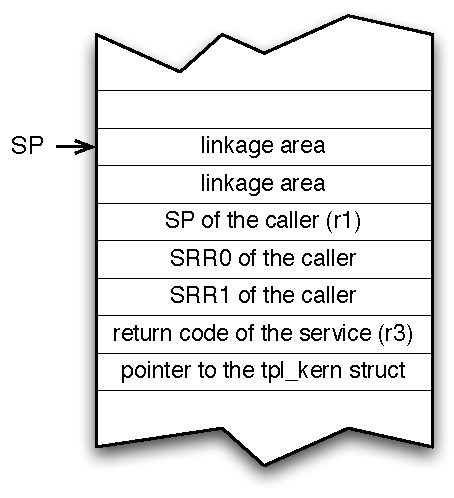
\includegraphics[scale=.6]{pictures/KStackMapping} 
\end{minipage}
\begin{minipage}{0.5\textwidth}
  \caption{Kernel stack mapping after allocation.}\label{fig:kernelstackmapping}
\end{minipage}
\end{figure}

\subsubsection{Calling the service}

Since the registers used to pass parameters to a function, that is \reg{r3} to \reg{r10} as documented in \cite{PPCeabi}, have not been changed until now, calling the function that implements the service respects the register usage conventions.

The first thing to do is to get the function pointer corresponding to the service id. The service id is in \reg{r0} as explained in \ref{sec:systemservices} and is used as an index to the \var{tpl_dispatch_table}.

\begin{lstlisting}[language=C]
  slwi  r0,r0,2                           /* compute the offset    */
  /*
   * load the ptr to the dispatch table
   */
  lis   r11,TPL_HIG(tpl_dispatch_table)     
  ori   r11,r11,TPL_LOW(tpl_dispatch_table)
  lwzx  r11,r11,r0                  /* get the ptr to the service  */
  mtlr  r11                         /* put it in lr for future use */
\end{lstlisting}

The second thing to do is to reset the \var{tpl_need_switch} flag that triggers a context switch. This flag (a byte) is located in the \var{tpl_kern} kernel struct. This is done as follow:

\begin{lstlisting}[language=C]
  lis   r11,TPL_HIG(tpl_kern)
  ori   r11,r11,TPL_LOW(tpl_kern)
  stw   r11,KS_KERN_PTR(r1)        /* save the ptr for future use  */
  li    r0,NO_NEED_SWITCH
  stb   r0,20(r11)
\end{lstlisting}

In the future \var{tpl_kern} will be reused, so its address is saved in the kernel stack.

Then, to allow reentrancy for a service call in a hook, the \reg{RI} bit of the \reg{MSR} is set to 1. Without that, a \asfct{sc} cannot be  properly executed.

\begin{lstlisting}[language=C]
  mfmsr r11
  ori   r11,r11,RI_BIT_1
  mtmsr r11
\end{lstlisting}

At last, the service is called:

\begin{lstlisting}[language=C]
  blrl
\end{lstlisting}

\subsubsection{Context switch}

The \var{tpl_need_switch} flag that as been possibly modified by the service is now checked to do a context switch if needed.

\begin{lstlisting}[language=C]
  lwz   r11,KS_KERN_PTR(r1) /* get back the tpl_kern address */
  lbz   r12,20(r11)         /* get the tpl_need_switch flag  */
  andi. r0,r12,NEED_SWITCH  /* check if a switch is needed   */
  beq   no_context_switch
\end{lstlisting}

A context switch is performed in 3 steps. The first one is the context save of the process that loses the CPU. This step is optional because if the service was a \api{TerminateTask} or a \api{ChainTask}, the context needs not to be saved. This information is in the \var{tpl_need_switch} flag. Before doing the actual context save, the return value of the service must be saved in the proper location of the kernel stack. The \cfunction{tpl_save_context} function will read it from this location and expects a pointer to the context saving area or the process in \reg{r3}. \var{s_old}, the address of the context saving area, is in another member of \var{tpl_kern}. At the end, the \var{tpl_kern} address is reread because \reg{r11} has been destroyed in \cfunction{tpl_save_context}. 

\begin{lstlisting}[language=C]
  stw   r3,KS_RETURN_CODE(r1) /* save the return value             */
  andi. r0,r12,NEED_SAVE      /* r12 contains tpl_need_switch      */
  beq   no_save
  lwz   r3,0(r11)             /* r11 contains the tpl_kern address */
  bl    tpl_save_context      /* and s_old is put into r3          */
  lwz   r11,KS_KERN_PTR(r1)   /* get back tpl_kern address         */
\end{lstlisting}

The second step consists in loading the configuration of memory protection for the process that get the CPU by calling the \cfunction{tpl_set_process_mp} function. This function expects the id of the process in \reg{r3}. Again this id is located in member \var{proc_id} of \var{tpl_kern}. This is done only if \cmacro{WITH_MEMORY_PROTECTION} is \YES. 

\begin{lstlisting}[language=C]
#if WITH_MEMORY_PROTECTION == YES
  lwz   r3,16(r11) /* get the id of the process which get the cpu  */
  bl    tpl_set_process_mp     /* set the memory protection scheme */
#endif
\end{lstlisting}

The third step loads the context of the process that get the CPU. The address of \var{tpl_kern} is loaded into \reg{r11} because it has been destroyed in \cfunction{tpl_set_process_mp}, \var{s_running}, the address of the context saving area of the current process is loaded into \reg{r3} and \cfunction{tpl_load_context} is called. At last, \reg{r3} is restored.

\begin{lstlisting}[language=C]
  lwz   r11,KS_KERN_PTR(r1)
  lwz   r3,4(r11)                    /* get s_running              */
  bl    tpl_load_context
  lwz   r3,KS_RETURN_CODE(r1)
\end{lstlisting}

\subsubsection{Switching back to the process stack}

At this stage, the \reg{SRR0} and \reg{SRR1} registers saved in the kernel stack are restored. The space reserved in the kernel stack is freed. The reentrancy counter is decremented and the stack switches to the process stack if the reentrancy counter is 0.

\begin{lstlisting}[language=C]
  lwz   r11,KS_SRR0(r1)
  mtspr spr_SRR0,r11
  lwz   r11,KS_SRR1(r1)
  mtspr spr_SRR1,r11

  addi  r1,r1,KS_FOOTPRINT       /*  free back space on the stack  */
  
  /*
   * The reentrency counter is decremented. If it reaches
   * 0, the process stack is restored
   */
  lis   r11,TPL_HIG(tpl_reentrancy_counter)
  ori   r11,r11,TPL_LOW(tpl_reentrancy_counter)
  lwz   r12,0(r11)    /*  get the value of the counter */
  subi  r12,r12,1
  stw   r12,0(r11)
  cmpwi r12,0
  bne   no_stack_restore

  /*  Restore the execution context of the caller
      (or the context of the task/isr which just got the CPU)      */
  lwz   r1,KS_SP-KS_FOOTPRINT(r1)   /*  Restore the SP and switch
                                        back to the process stack  */
\end{lstlisting}

\subsubsection{Enabling memory protection}

Then, if memory protection is used, the user scheme is reenabled. The actual works depends on the kind of MPU and is done in \cfunction{tpl_user_mp}.

\begin{lstlisting}[language=C]
#if WITH_MEMORY_PROTECTION == YES
  subi  r1,r1,4
  mflr  r11
  stw   r11,0(r1)   /* save lr on the current stack  */
  bl    tpl_user_mp /* Enable the memory protection  */
  lwz   r11,0(r1)   /* restore lr                    */
  mtlr  r11
  addi  r1,r1,4
#endif
\end{lstlisting}

\subsubsection{Restoring registers}

Registers saved at stage 1 on the process stack are restored an the stack is freed.

\begin{lstlisting}[language=C]
  lwz   r11,PS_CR(r1)
  mtcr  r11
  lwz   r11,PS_LR(r1)
  mtlr  r11
  lwz   r12,PS_R12(r1)
  lwz   r11,PS_R11(r1)

  addi  r1,r1,PS_FOOTPRINT
\end{lstlisting}

\subsubsection{Getting back to the process}

At last, the dispatch layer is exited using a \asfct{rfi}.

\begin{lstlisting}[language=C]
  rfi                                 /* return from interrupt */
\end{lstlisting}

\subsection{Interrupt handler}

\subsection{The CallTrustedFunction service}

The \api{CallTrustedFunction} service is implemented by the \cfunction{tpl_call_trusted_function_service} function. This function is a special case of service because the kernel stack and the process stack have to be modified. In addition, an \api{ExitTrustedFunction} service is implemented to restore the process stack when the trusted function exits. Both services have to be written in assembly language since C does not allow to explicitely modify the stack.

\cfunction{tpl_call_trusted_function_service} performs the following steps:

\begin{penum}
\item check the trusted function id is within the allowed range
\item increment the trusted counter of the calling process
\item build a frame on the process stack to store the registers pushed by a service call except for \reg{r0} and for \reg{SRR0} and \reg{SRR1}; put the address of \api{ExitTrustedFunction} in the \reg{lr} location in the process stack; save \reg{SRR0} and \reg{SRR1} in the process stack
\item get the trusted function address and put it in \reg{SRR0}
\item go back to the dispatch layer
\end{penum}

\subsubsection{Checking the trusted function id}

The id of the trusted function is checked to avoid to call a function at an arbitrary address.

\begin{lstlisting}[language=C]
mov   r11,r3               /* save r3 in r11 b/c it will be destroyed */
cmpw  r3,TRUSTED_FCT_COUNT /* check the id of the trusted function    */
ori   r3,r0,E_OS_SERVICEID /* E_OS_SERVICEID return code              */
bge   invalid_trusted_fct_id
mov   r3,r11               /* restore r3 if trusted function id ok    */
\end{lstlisting}

\subsubsection{Incrementing the trusted counter}

The trusted counter of the process is incremented each time a trusted function is called. When the trusted counter is $>0$, the process is trusted. In such a case, the dispatch layer does not enable memory protection when scheduling the process so it has an unlimited access to the whole addressing space.

\begin{lstlisting}[language=C]
  lwz   r11,KS_KERN_PTR(r1) /* get the ptr to tpl_kern                  */
  lwz   r11,12(r11)         /* get the ptr to the runnning process desc */
  lwz   r12,4(r11)          /* get trusted_count member                 */
  addi  r12,r12,1           /* increment it                             */
  stw   r12,4(r11)          /* put it back in the process desc          */
\end{lstlisting}

\subsubsection{Building the frame}

The frame is used to store the calling context of the trusted function and is shown in figure \ref{fig:tfstackmapping}. The following code builds this frame:

\begin{lstlisting}[language=C]
  /*
   * First get back the process stack pointer
   */
  lwz   r11,KS_SP(r1)
  /*
   * Make room to prepare the call of the trusted function
   */
  subi  r11,r11,PS_TRUSTED_FOOTPRINT_IN
  /*
   * store ExitTrustedFunction as the return address
   */
  lis   r12,TPL_HIG(ExitTrustedFunction)
  ori   r12,r12,TPL_LOW(ExitTrustedFunction)
  stw   r12,PS_LR(r11)
  /*
   * Update the stack pointer
   */
  stw   r11,KS_SP(r1)
  /*
   * second get back SRR0 and SRR1 and save them to the process stack
   */
  lwz   r12,KS_SRR0(r1)
  stw   r12,PS_SRR0_IN(r11)
  lwz   r12,KS_SRR1_IN(r1)
  stw   r12,PS_SRR1(r11)
\end{lstlisting}

\begin{figure}[htbp] %  figure placement: here, top, bottom, or page
\begin{minipage}{0.65\textwidth}
    \centering
  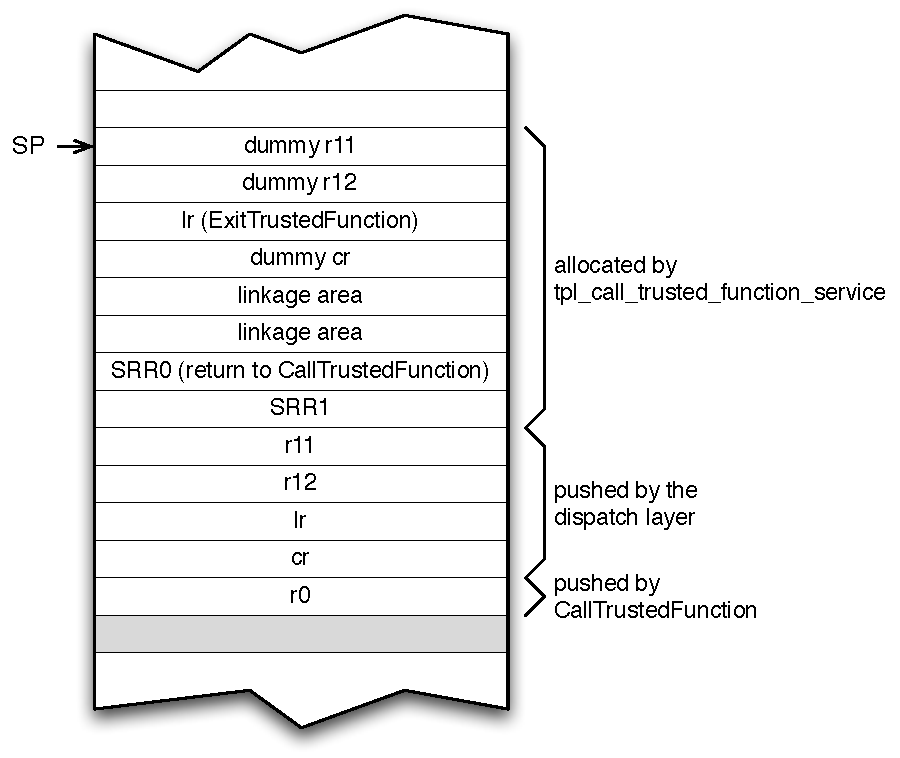
\includegraphics[scale=.6]{pictures/TFStack1} 
\end{minipage}
\begin{minipage}{0.35\textwidth}
  \caption{Process stack mapping at the end of \cfunction{tpl_call_trusted_function_service}. \reg{r0}, at the bottom of the stack has been pushed by \api{CallTrustedFunction}. \reg{cr} to \reg{r11} has been pushed by the dispatch layer. \reg{SRR0} and \reg{SRR1} are saved here by \cfunction{tpl_call_trusted_function_service} to be able to go back to the calling process. Above, the linkage area allows the trusted function to call functions. Above, a frame that will be used by the dispatch layer to restore an execution context for the trusted function is built.}\label{fig:tfstackmapping}
\end{minipage}
\end{figure}

\subsubsection{Setting the trusted function address}

The \reg{SRR0} saved by the dispatch layer after the \api{CallTrustedFunction} is changed to the address of the trusted function. This way, instead of returning to the caller, the trusted function will be executed.

\begin{lstlisting}
  lis   r11,TPL_HIG(tpl_trusted_fct_table)
  ori   r11,r11,TPL_LOW(tpl_trusted_fct_table)
  slwi  r0,r3,2
  lwzx  r12,r11,r0
  stw   r12,KS_SRR0(r1)
\end{lstlisting}

\subsubsection{Going back to the dispatch layer}

A simple \asfct{blr} goes back to the dispatch layer. The latter cleans up the process stack. Once the trusted function starts execution, the process stack is like that:

\begin{figure}[htbp] %  figure placement: here, top, bottom, or page
\begin{minipage}{0.5\textwidth}
    \centering
  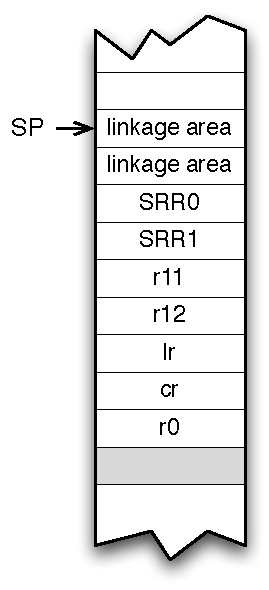
\includegraphics[scale=.6]{pictures/TFStack2} 
\end{minipage}
\begin{minipage}{0.5\textwidth}
  \caption{Process stack mapping when the trusted function starts its execution.}\label{fig:tfstackmapping2}
\end{minipage}
\end{figure}

\subsection{The ExitTrustedFunction service}\label{sec:exittfppc}

When a trusted function finishes, the context of the \api{CallTrustedFunction} must be restored to return to the caller. \api{ExitTrustedFunction} does not need to be called explicitly because its address has been set as the return address of the trusted function by \cfunction{tpl_call_trusted_function_service}. Calling \api{ExitTrustedFunction} explicitly may result in an undefined behavior or in the crash of the calling process but see below. The mapping of the process stack at start of \cfunction{tpl_exit_trusted_function_service} is shown in figure \ref{fig:ETFstack1}.

\begin{figure}[htbp] %  figure placement: here, top, bottom, or page
\begin{minipage}{0.4\textwidth}
    \centering
  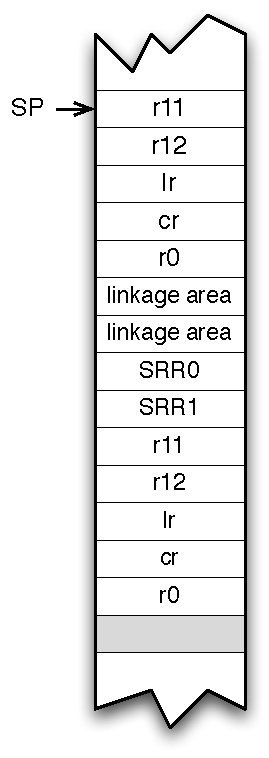
\includegraphics[scale=.6]{pictures/ETFStack1} 
\end{minipage}
\begin{minipage}{0.6\textwidth}
  \caption{Process stack mapping when the \cfunction{tpl_exit_trusted_function_service} function starts its execution.}\label{fig:ETFstack1}
\end{minipage}
\end{figure}

First, \cfunction{tpl_exit_trusted_function_service} decrements the trusted counter of the calling process. A particular attention must be given to this point because by building a fake stack frame and calling Explicitly \api{ExitTrustedFunction} to underflow this counter, a process could get a full access to the memory. So the counter is tested before to avoid to go under 0.

\begin{lstlisting}[language=C]
  lwz   r11,KS_KERN_PTR(r1) /* get the ptr to tpl_kern */
  lwz   r11,12(r11)         /* get the ptr to the runnning process desc */
  lwz   r12,4(r11)          /* get trusted_count member */
  /*
   * Warning, the trusted counter has to be check (compared to 0) to
   * avoid to decrement it if it is already 0. Without that a process
   * could build an had-hoc stack an call explicitly ExitTrustedFunction
   * to get access to all the memory.
   */
  cmpwi r12,0               /* check it is not already at 0 */
  beq   cracker_in_action   /* uh uh */
  subi  r12,r12,1           /* decrement it */
  stw   r12,4(r11)          /* put it back in the process desc */
\end{lstlisting}

\cfunction{tpl_exit_trusted_function_service} has to remove from the process stack the frame that was built by \cfunction{tpl_call_trusted_function_service}, restore \reg{SRR0} and \reg{SRR1} before returning to the dispatch layer.

\begin{lstlisting}[language=C]
cracker_in_action:
  
  /*
   * get the process stack pointer
   */
  lwz   r11,KS_SP(r1)
  
  /*
   * get back the SRR0 and SRR1
   */
  lwz   r12,PS_SRR0_OUT(r11)
  stw   r12,KS_SRR0(r1)
  lwz   r12,PS_SRR1_OUT(r11)
  stw   r12,KS_SRR1(r1)
  
  /*
   * free the process stack and update it in the kernel stack
   */
  addi  r11,r11,PS_TRUSTED_FOOTPRINT_OUT
  stw   r11,KS_SP(r1)
  
  /*
   * that's all
   */
  blr
\end{lstlisting}

\subsection{Execution of the OS Applications startup and shutdown hooks}

These hooks are executed from the kernel but with the access right of a task belonging to the OS Application. The \sysgen\ should choose one of the tasks of the OS Application to be used as context to execute the OS Application startup and shutdown hooks. Execution of an OS Application startup hook is done by the \cfunction{tpl_call_startup_hook_and_resume} function. The argument of this function is a function pointer to the hook. Similarly execution of an OS Application shutdown hook is done by the \cfunction{tpl_call_shutdown_hook_and_resume} function. These functions end by a call to \api{NextStartupHook} and \api{NextShutdownHook} services respectively to cycle through the hooks.

\subsection{The MPC5510 Memory Protection Unit}

The access control rights of the memory region descriptor rules the access of 5 bus masters (labeled from 4 to 0). Unused bus masters are set to the same access right for all the regions. Bus master 4 is used for factory testing only, so the access rights should be set to no access. Bus master 3 is the Flexray controller. Since it is not used in the current version of Trampoline, it is set to no access too. Bus master 2 is the DMA controller and for the same reason it is set to no access. Bus master 1 is the Z0 core. Again it is set to no access.

The access control rights register has the following bit usage:

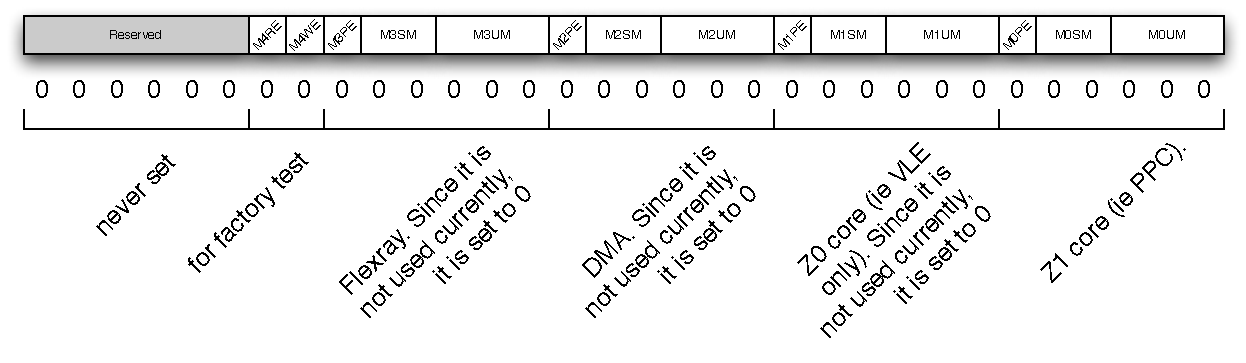
\includegraphics[width=\textwidth]{pictures/MPUacr.pdf} 

Bus master 4 is a special case. The 2 bits have the following meaning:

\rowcolors{1}{white}{light-gray}
\begin{longtable}[c]{l|p{5.15in}}
{\bf Bit}&{\bf Meaning}\\
\hline
\dreg{M4RE} & If set to 1, bus master 4 may {\bf read} memory in the region. If 0, no read is allowed\\
\dreg{M4WE} & If set to 1, bus master 4 may {\bf write} memory in the region. If 0, no write is allowed\
\end{longtable}

So in our case, these bits are set to 0.

Of course, other bus masters have more sophisticated access right:

\rowcolors{1}{white}{light-gray}
\begin{longtable}[c]{l|p{5.15in}}
{\bf Bit}&{\bf Meaning}\\
\hline
\dreg{MxPE} & The PID Enable bit. Set to 0 in our case\\
\dreg{MxSM} & These 2 bits rules the supervisor mode access control with the following meaning: $00=rwx$, $01=rx$, $10=rw$, $11=$ \textit{same as defined by \dreg{MxUM}}. In our case, it is set to $00$ for code and constants and to $11$ for data.\\
\dreg{MxUM} & These 2 bits rules the user mode access control. The first bit means $r$, the second one $w$ and the third one $x$.
\end{longtable}

Trampoline uses 4 descriptors:

\rowcolors{1}{white}{light-gray}
\begin{longtable}{l|p{1.9in}|p{2.6in}}
{\bf Descriptor} & {\bf Usage} & {\bf \dreg{MxUM} value}\\
\hline
\dreg{MPU_RGD0} & Constants and program\footnote{This region is set to the whole addressing space. This is not definitive and should be improved because reading a peripheral control register should be protected. So an additional descriptor has to be used to allow the kernel (supervisor mode) a complete access on all the memory space and no access at all for applications (user mode).}. & $rwx=00$ for supervisor mode, $rx=101$ for user mode.\\
\dreg{MPU_RGD1} & Private variables of the process. & $rw=110$ for supervisor and user mode.\\
\dreg{MPU_RGD2} & Stack of the process. & $rw=110$ for supervisor and user mode.\\
\dreg{MPU_RGD3} & Variables of the OS Application if OS Applications are used. & $rw=110$ for supervisor and user mode.\\
\end{longtable}

So values of access control bits should be:

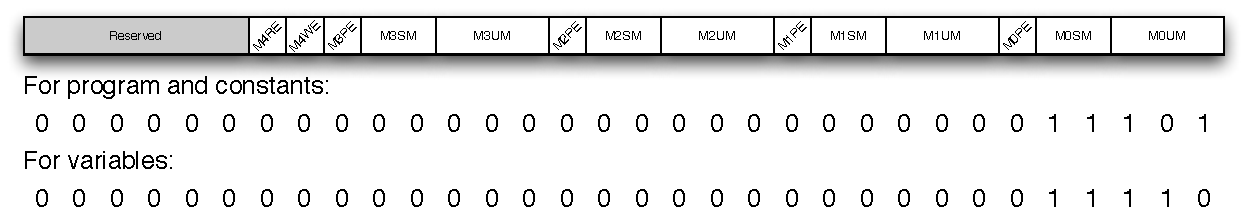
\includegraphics[width=\textwidth]{pictures/MPUprog.pdf} 

So in hexa:

\rowcolors{1}{white}{light-gray}
\begin{longtable}{l|l}
{\bf Kind} & {\bf Value}\\
\hline
Program region access & $0x00000005$\\
Variable region access & $0x0000001E$\\
\end{longtable}

\subsubsection{What happen in case of memory protection violation ?}

Two exception handler are used to handle a memory protection violation, one for data access, one for code access.

The Data Storage exception is tied to the IVOR~2 vector (VPR offset = 0x020), see page 8-2 of the {\em MPC5510 Microcontroller Family Reference Manual}.

The Instruction Storage exception is tied to the IVOR~3 vector (VPR offset = 0x030), see page 8-2 of the {\em MPC5510 Microcontroller Family Reference Manual}.

However, it appears one of these exceptions is raised when the processor is in user mode. The behavior is different in supervisor mode {\em to be completed}.

\section{ARM -- Common conventions}

\subsection{File hierarchy}

\subsection{Common definitions}

\subsection{Bootstraping}

The bootstrap must be made in specific ARM port and must call the \cfunction{main} function. If \cfunction{main} ever returns, the bootstrap code must fall into an infinite loop.

As a reason, many ARM architectures needs early specific and required initializations. This includes steps like memory mapping configuration, DRAM controller configuration, ...

Besides specific initializations, the bootstrap should :
\begin{itemize}
\item initialize stack pointer for every ARM exception modes
\item keep all external interrupts locked (will be unlocked at the first task context loading)
\item call \cfunction{main} in "system" mode (0x1F)
\end{itemize}

\subsection{Stacks}

\subsection{Interrupt management}

Kernel is not interruptible. So hardware interrupt source are disabled entering in kernel (via any case in system call, interrupt request, abort, ...).

But kernel shall be reentrant via system call (because kernel hooks can call some system calls).

\subsubsection{Interrupt and category classification}

All ARM IRQ are category 2 ISR.

All ARM FIQ are category 1 ISR.

\subsubsection{Vector table}

Each ARM exception vector points on a so called "primary" subprogram (like \cfunction{tpl\_primary\_syscall\_handler}).

To be located at address 0x00000000, this vector table is assigned to a specific section named \cfunction{.vectbl}. The linker script uses this section name to output it to address 0x00000000.

\subsubsection{System call}

\subsubsection{IRQ handling}

\subsubsection{FIQ handling}

\section{ARM -- Armadeus APF27 board}

\subsection{Debugging with Abatron BDI2000 or BDI3000 JTAG probe}

A configuration file is provided in \file{machines/arm/armadeus-apf27/bdi-config}.

To enable JTAG, if your APF27 has a FPGA, you must load the FPGA to wake it up (TO DO : explain how to do this...).

To start a debug session, follow these steps :
\begin{enumerate}
\item connects everything together
\item power up everything
\item reset the APF27 (S2 on APF27-Dev)
\item stop u-boot before it loads Linux (if MMU is started, you won't be able to load anything)
\item telnet your BDI
\item type \cfunction{reset} command in the BDI shell
\item start GDB session (\cfunction{target remote ...})
\end{enumerate}

\subsection{Configuration}

All configuration of port is done in \file{apf27\_config.h}.

\subsubsection{Stacks}

Stacks' size (stack of each exception mode) can be adjusted via the following constants. Remember that the size must be aligned to 4.

\subsubsection{CPU caches}

By default, CPU caches are disabled (for real time determinism).

\subsection{Memory mapping}

This port can be use in one of these three configurations :
\begin{enumerate}
\item No memory mapping (and thus no memory protection)
\item Memory mapping without memory protection
\item Memory mapping and memory protection
\end{enumerate}

\subsection{Memory protection}

To be written...

Some points to explain :
\begin{itemize}
\item FCSE mechanism is not used by this port (if someone is interested by this work, she's welcome)
\item address translation is not used, all VMA equals physical address
\item IDLE task's memory protection configuration is used to provide configuration for trusted applications or kernel
\end{itemize}

\subsubsection{MMU tables generation principle}

To be written...

Some points to explain :
\begin{itemize}
\item MMU is not disabled in privileged mode, but all useful memory areas are accessible. Thus, we hope we can find bugs easily in privіleged code.
\item useful memory areas, except processes and applications ones, are configured as accessible (read and write) in privileged mode. These memory areas are called system areas
\item some memory areas needs to be accessible by anyone (API, GCC builtin functions, common libraries, ...), they are called common areas (they are read only for unprivileged contexts)
\item there is one translation table for each process
\item all translation tables have the same system and common areas
\item there is one page table set for each process. Page tables are fine page tables. Table entries are tiny page descriptors.
\item the number of page table in a set depends on the size of the whole trampoline and application memory footprint. Then this information is given by linker via a symbol which is used by the MMU driver.
\item Page tables are accessed via a macro, as they are allocated by linker (and we cannot know the number of page tables)
\end{itemize}

\section{ARM -- Simtec EB675001 board}

\subsection{Memory map and hardware resources}

Talk about configured memory map (use of DRAM, where the bootstrap would be flashed, \ldots).

Tell which hardware resources are used by the kernel.

\subsection{Booting}

There is two way to start Trampoline on APF27 :
\begin{itemize}
\item from ELF image (in file usually called \file{trampoline})
\item from raw binary image (in file usually called \file{trampoline.bin})
\end{itemize}

\subsubsection{Booting from ELF image}

Load image with your ELF loader (the file is usually named \file{trampoline}). This can be GDB via a JTAG probe for example. Then, just start execution from \cfunction{tpl\_arm\_bootstrap\_entry} entry point. Here are commands you can type in GDB :
\begin{lstlisting}
(gdb) load
(gdb) set $pc=tpl_arm_bootstrap_entry
(gdb) break main
(gdb) continue
\end{lstlisting}

\subsubsection{Booting from raw binary image}

Load image with your binary loader to 0xA0000000 memory address. Then just start execution at this point (0xA0000000).

With u-boot, you can type these commands :
\begin{lstlisting}
BIOS> tftpboot 0xA0000000 192.168.5.20:trampoline.bin
BIOS> go 0xA0000000
\end{lstlisting}

\subsection{Internal kernel drivers}

\subsection{Hardware interrupts handling}

\subsection{Idle task}

\subsection{Exceptions handling}


\subsection{Kernel sleep service}

